\documentclass[11pt]{article}

\usepackage{alltt,fullpage,graphics,color,epsfig,amsmath, amssymb}
\usepackage{hyperref}
\usepackage{boxedminipage}
\usepackage[ruled,vlined]{algorithm2e}

\newcommand{\floor}[1]{\lfloor #1 \rfloor}
\newcommand{\ceil}[1]{\lceil #1 \rceil}

\title{Algorithmic Game Theory HW2}
\author{Daniel Campos}
\date{October 30th, 2020}
\begin{document}

\maketitle
\begin{enumerate}
\section{Problem 1}
%----------------------------------------------------------------------
\item 
\begin{enumerate}
    \item (3 points) The following game has a unique Nash equilibrium. Find
it, and prove that it is unique. (Hint: look for strict dominance.)
\begin{center}
\begin{tabular}{| c | c | c | c|}
\hline
\textbf{Strategy} & \textbf{X} & \textbf{Y} & \textbf{Z} \\ \hline \hline
\textbf{A} & 4, 0 & 1, 1 & 4, 0 \\ \hline
\textbf{B} & 1, 3 & 2, -1 & 3, 5 \\ \hline
\textbf{C} & 0, 1 & 3, 0 & 3, 0 \\
\hline
\end{tabular}
\end{center}
\subsection{Solution}
We begin by seeking a strict dominance. Since there is no single strategy strict dominance we search for a mixed strategy strict dominance.
\begin{enumerate}
    \item For the mixed strategy A + C assume player 1 chooses strategy A with probability $p$ and strategy C with probability $1-p$ we find the following expected outcomes For player 2s strategy X $4(p) + 1(1-p)= 4p +1 -p = 3p +1$ which is > 1 which is the result of strategy B. For player 2s strategy Y $1(p) + 3(1-p) = p + 3 - 3p = 3 - 2p$ which for $p \le 0.5$ is equal or better to strategy B. For player 2s strategy Z $4(p) + 3(1-p) = 4p+3-3p=3+p$ which for $p \ge 0$ is an equal or better strategy than B. Thus mixed strategy A + C strictly dominates strategy B.
    \item For player 2 now that player 1 will not play strategy B their strategy Z is strictly dominated by X and Y since strategy Z only produces no gains. This leaves us with the table below. 
    \item
    \begin{tabular}{| c | c | c |}
    \hline
    \textbf{Strategy} & \textbf{X} & \textbf{Y} \\ \hline \hline
    \textbf{A} & 4, 0 & 1, 1 \\ \hline
    \textbf{C} & 0, 1 & 3, 0 \\ \hline
    \end{tabular}
    \item In the table above we find no single strategy strict dominant equilibrium so once again we look for mixed strategies. Let the probability that player 1 chooses strategy  A be $p$ and the probability the choose strategy B $1-p$. We set the $E_x = E_y$ and since $E_x = 4*p + 0(1-p) = 4p + 0$ and $E_y = 1(p) + 3(1-p) = 3 - 2p$ thus $4p = 3 - 2p$ which simplifies to $6p = 3$ meaning $p=\frac{1}{2}$.
    \item Similarly let the probability that player 2 chooses strategy X be $q$ and the probability they choose strategy Y $1-q$. $E_a = 0*q + 1(1-q) = 1 -q$ and $E_c = 1*q + 0(1-q) = q$ and since $E_c = E_a$ $1 - q = q$ which simplifies to $1 = 2q$ meaning $q = \frac{1}{2}$. 
    \item Since $q = \frac{1}{2}$ and $p = \frac{1}{2}$ AX, AY, CX, and CY are Nash equilibriums each with a probability $\frac{1}{4}$
\end{enumerate} 

\item (4 points). Construct a single $2 \times 2$ normal-form game that simultaneously
has all four of the following properties:
\begin{enumerate}
\item The game does not have a dominant strategy Nash equilibrium (at least one player does not have a dominant strategy).
\item The game is solvable by iterated weak dominance (so that one pure strategy per player remains).
\item In addition to the iterated weak dominance solution (which is a Nash
equilibrium), there is a second pure-strategy Nash equilibrium.
\item Both players strictly prefer the second equilibrium to the first.
(Hints: the second pure-strategy equilibrium should not be strict; the pure strategy equilibria should be in opposite corners of the matrix.) If you cannot get all four properties, construct an example with as many of the properties as you can.
\end{enumerate}
\subsection{Solution}
\begin{center}
\begin{tabular}{| c |  c | c |}
\hline
\textbf{Strategy} & \textbf{X} & \textbf{Y}\\ \hline \hline
\textbf{a} & 1, 1 & 5, 3 \\ \hline
\textbf{b} & 4, 2 & 6, 1 \\ \hline
\end{tabular}
\end{center}
\begin{enumerate}
\item We meet not having a dominant strategy because  player 2(who plays rows) does not have a dominant strategy.
\item We meet the second criteria since player 1 has a dominant strategy and will always play strategy b. Since player 1 will always play strategy b player 2 will chose to play strategy X and the NE is 4,2.
\item We meet the third criteria and fourth criteria because we have a second pure-strategy NE of 5,3 which is opposite the iterate weak dominance NE. If both players had pure strategy then they would chose strategy Y and B giving them the maximum reward of 5,3.
\end{enumerate}
\item (3 points). Consider the following game:
\begin{center}
\begin{tabular}{| c | c | c |}
\hline
\textbf{Strategy} & \textbf{X} & \textbf{Y}\\ \hline \hline
\textbf{a} &2, 5 & 1, 5 \\ \hline
\textbf{b} &7, 1 & 0, 0 \\
\hline
\end{tabular}
\end{center}
Find a correlated equilibrium that places positive probability on all entries of the matrix, except the lower-right hand entry. Try to maximize the probability in the upper-left hand entry.
\end{enumerate}
\subsection{Solution}
First Assume a third party draws one of three cards labeled (A,X), (A, Y), or (B,X) with the probabilities $\frac{4}{8}$ , $\frac{3}{8}$, $\frac{1}{8}$. After drawing the card the third party informs the players of the strategy assigned to them on the card (but not the strategy assigned to their opponent). For player 1(playing rows) the expected utility of strategy a is $2*\frac{1}{2} + 1*\frac{1}{2} = 1.5$ and the expected utility of strategy b is $7*\frac{1}{2} + 0*\frac{1}{2} = 3.5$ meaning they would prefer strategy b. For player 2(playing columns) the expected utility of strategy x is $5*\frac{1}{2} + 1*\frac{1}{2} = 3$ and the expected utility of strategy y is $2*\frac{1}{2} + 0*\frac{1}{2} = 2.5$ so they prefer strategy X. If they play the card they are assigned player 1 has a expected utility of $2*\frac{1}{2} + 7*\frac{3}{8} + 1*\frac{1}{8} = \frac{30}{8} = 3.75$ and player 2 has a expected utility of $5*\frac{1}{2} + 1*\frac{3}{8} + 5*\frac{1}{8} = \frac{28}{8} = 3.5$. Since neither player has an incentive to deviate, this is a correlated equilibrium with the highest probability being in the upper left hand entry.
\item Consider a symmetric $2$ person game between Alice and Bob, with the same strategy set $S$ for both players. Let $A(i, j)$ and $B(i,j)$ denote the payoff of Alice and Bob respectively, when Alice plays $i$ and Bob plays $j$. We say that the game is symmetric if we have that $A(i,j) = B(j,i)$ for all $i,j \in S$, {\em i.e.,} $B=A^T$.
\section{Problem 2}
\begin{enumerate}
    \item (2 points) Can a symmetric game have a pure Nash equilibria? (even if all values $A(i,j)$ are different?)
    \subsection{Solution}
    Yes. Take the prisoners dilemma as an example. One of the pure strategies is Betray, Betray. Both players betraying is a nash equilibria because both players are always better off betraying regardless of the other players choice. 
    \item (2 points) Do all symmetric games have pure Nash equilibria?
    \subsection{Solution}
    No. Take Rock Paper Scissors as an example. It is a  three strategy symmetric game with no pure-strategy equilibrium. None of the six pure strategies (RR, RP, RS, PP, PS, SS) are equilibria. The same goes for a game like the penny matching game where two players choose an action heads or tails. Player 1 wins if there is a match, player 2 if there is not. None of the pure-strategy profiles (HH,TT,HT,TH) constitute an equilibrium.
    \item (6 points) J. Nash showed that every symmetric game has a symmetric equilibrium, i.e., a probability distribution $x\in \Delta(S)$ such that $(x,x)$ is an Nash equilibrium. Using this fact derive a quadratic program to compute a symmetric equilibrium of game $(A,A^T)$. 
    \subsection{Solution}
    First we must define what a the nash equilibria are in matrix form. A nash equilibra for the game is a pair of strategies $(x, y) \in \delta_i \delta_j$ such that $x^{T} A y \ge x A y ,\forall x \in \delta_i$ and $x^{T} A^{T} y \ge x A^{T} y ,\forall x \in \delta_j$. \\
    Given that nash prove that that symmetric equilibrium are probability distributions we formalize this problem as a quadriatic feasability problem. 
    
    \begin{equation}
    \begin{split}
    \min_{x \in \mathbb{R}^i, y \in \mathbb{R}^j} \; 0 \; \\ subject \; to \; x^{T} A y \ge x A y ,\forall x \in {1,...,i}, \\
    x^{T} A^{T} y \ge x A^{T} y ,\forall y \in {1,...,j}, \\
    x_i \ge 0, \forall i \in {1,...,i}, \\
    y_i \ge 0, \forall j \in {1,...,j}, \\
    \sum_{m=1}^{i}x_m = 1, \\
    \sum_{n=1}^{j}y_n = 1.
    \end{split}
    \end{equation}
\end{enumerate}
\section{Problem 3}
\item The $1$-dimensional Sperner's problem is defined on a 1-dimensional grid from $[0, 2^n-1]$, with each integer being a grid point. There are two colors, red and blue, represented by $0$ and $1$ respectively. 
There is a Boolean circuit named {\em Color,} which outputs the color ($0$/$1$ bit) of a grid point given its bit representation, such that,
Color($0$) = red, Color($2^n-1$) = blue, and the remaining grid points get any color.

\begin{enumerate}
    \item (4 points) Show that there exists an integer $0\le k \le 2^n-1$ such that Color($k$)=red and Color($k+1$)=blue. Furthermore, we can compute it in $O(n)$ calls to the Boolean circuit ``Color''.
    \subsection{Solution}
     To rephrase we know that essentially there is a discrete function that can create the 1d grid which produces values 0 and 1. Since it begins with 0 and ends with 1 then it much switch values an odd number of times. As such there is at least 1 integer k where this switch occurs and Color(k) = red and color(k+1) = blue. To find k we only need O(n) calls to the boolean circuit because at each call we essentially learn two things. If for spot k $0 \ge k \ge 2^n-1$ we call color(k) and we get blue we know that somewhere between [1,k] there has been a switch to blue and thus only need to further search in range [1,k-1]. If we call color(k) and the color is red we know that either we have not passed the switch point or there is at least one more switch between $[k+1,2^n-1]$. As a result we are essentially doing a binary search which is o(log(x)) and since our $x=n^2-1$ our search time is $< O(n-1) -1 $ since we know start and end(2 points) and our x value.
    \item (6 points) Show that checking if there are more than one such $k$s is NP-complete (hint: reduce from 3-SAT).
    \subsection{Solution}
    To solve this we make this a 3-SAT problem by setting up the representation that a point $k = (x_1 	\land x_2 	\land x_3)$ where $x_1$ is color(k) = red, $x_2$ is color(k+1) = blue and $x_3$ is $ 0 \le k \le 2^n -1$. We must do this for every point in $[0,2^n-1]$ as a result we set up a graph where each each one of the 3 satisfy able variables is a vertex. Then if this value i is a k value then there will be an independent set of size k. Since we have to run this for every step in the grid the run time is np complete.
\end{enumerate}
\section{Problem 4}}
\item (10 points) In the town of Gamica, there is exactly one police patrol, two police stations ($s$ and $t$), and one robber. The robber plans to target a house on one of the streets at night, say on street $i\in [n]$. If street $i$ is patrolled by the police then they get $r_i$ reward while the robber gets $\zeta_i$ cost, otherwise police's cost is $c_i$ and the robber's reward is $\rho_i$. 

Every night, the police can patrol exactly one route from station $s$ to station $t$. \textcolor{red}{At night all the streets are one way, and the street network forms a DAG}. Design a polynomial time algorithm to compute Stackelberg strategy of the police. \\

{\em (Hint: What is the corresponding DBR problem? Can that be solved in polynomial time?)}
Defender's Best Response
\subsection{Solution}
First off, I will start on declaring my assumptions. First assumption is that the robber will be at the house they are targeting all night and thus it does not matter when the police pass the house but only that the robbed house is on their path from s to t. The next assumption is the robber has no notion of previous day's path. Since the optimization goal is to pick the longest path from s to t police do not have incentive to change their strategy day to day. If a robber had a notion of the previous days route they would just chose something off the longest path. \\
Following those assumptions the stackelberg strategy of the police is to find the longest path in the DAG from s to t so that they can cover the most houses. The reason this is the stacklberg strategy is the police are trying to optimize how many houses they can cover on their patrol and the way to maximize this is to take the longest path possible between the two stations. To find the longest distance we use algorithm \ref{algo1} and then we use algorithm  \ref{algo2} to find paths that match the longest length. We select from the longest paths one at random so the robber cannot predict. \\
\begin{algorithm}[H]
\SetAlgoLined
\KwResult{Longest Path distance finder}
\hspace*{\algorithmicindent} \textbf{Input:}Weighted DAG G = (V,E) \\
\hspace*{\algorithmicindent} \textbf{Output:} Largest path cost in G \\
Topologically sort G \\
\For{vertex $v \in V$} {
    $dist(v) = max_{(u,v) \in E} \{dist(u) + w(u,v)$\} }
\textbf{return} $max_{v \in V} \{dist(v)}$
 
 \caption{Longest Path Distance Finder}
 \label{algo1}
\end{algorithm}\\
\begin{algorithm}[H]
\SetAlgoLined
\KwResult{Police Patrolling Path}
\hspace*{\algorithmicindent} \textbf{Input:}all paths from s to t $P = [(s,v_1),(v_1,v2), ...,(v_n,t)]$ \\
\hspace*{\algorithmicindent} \textbf{Output:}max-distance = algorithm1 \\
possible-paths = []\\
\For{$p \in P$} {
    \If{$len(p) == max-distance$}{
        possible-paths.add($p$)
    } }
\textbf{return} possible-paths[random-number(0,len(possible-paths))]
 \caption{Path Finder version1}
 \label{algo2}
\end{algorithm}\\
If instead we assume that the polices preferences are common knowledge we must add some randomization to ensure that robber does not stay off the longest path. To ensure that police don't only follow the longest path we introduce a approximation variable $\epsilon$. Instead of search for the longest path the police offices look for all paths within $\epsilon$ of the longest path and then select one of these paths at random. $\epsilon$ is a learned parameter and must be defined based on the actual DAG size and the desired policing behavior. Our modified stackleber strategy is shown in algorithm \ref{algo3}. \\
\begin{algorithm}[H]
\SetAlgoLined
\KwResult{Police Patrolling Path}
\hspace*{\algorithmicindent} \textbf{Input:}all paths from s to t $P = [(s,v_1),(v_1,v2), ...,(v_n,t)]$ , $\epsilon$ \\
\hspace*{\algorithmicindent} \textbf{Output:}max-distance = algorithm1 \\
possible-paths = []\\
\For{$p \in P$} {
    \If{$len(p) + \epsilon \ge max-distance$}{
        possible-paths.add($p$)
    } }
\textbf{return} possible-paths[random-number(0,len(possible-paths))]
 \caption{Path Finder version1}
 \label{algo3}
\end{algorithm}\\
Both of these implementations are polynomial time.
\section{Problem 5}
\item Consider the extensive-form game shown in the figure.

\begin{figure}[!ht]
\centering
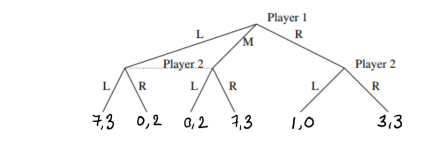
\includegraphics[width=0.5\textwidth]{hw2-Figure.png}
\caption{An extensive-form game with imperfect information.}
\end{figure}

\begin{enumerate}
    \item (3 points). Give the normal-form representation of this game.
    \subsection{Solution}
    Let player one represented by rows and player 2 by columns
    \begin{center}
    \begin{tabular}{| c | c | c |}
    \hline
    \textbf{Strategy} & \textbf{L} & \textbf{R} \\ \hline \hline
    \textbf{L} &  7,3 & 0,2\\ \hline
    \textbf{M} &  0,2 &  7,3 \\ \hline
    \textbf{R} &  1,0 & 3,3  \\ \hline
    \end{tabular}
    \end{center}
    \item (3 points). Give a Nash equilibrium where player $1$ sometimes plays left. (Remember that you must specify each player's strategy at {\em every} information set.)
    One such equilibrium is Player 1 has a mixed strategy of $\frac{1}{2}$ for L and $\frac{1}{2}$  for R with an expected value of 3.5 and player 2 has a mixed strategy of $\frac{1}{2}$ L and $\frac{1}{2}$  R with an expected value of 2.50
    \subsection{Solution}
    \item (4 points). Characterize the subgame perfect equilibria of the game. (Remember that you must specify each player's strategy at {\em every} information set.)
    \subsection{Solution}
    This game has two sub-games: player 2 choice after player 1 plays their choice, and the entire game. For the sub game after player 1 has chosen there are 3 perfect equilibria. When player 1 plays L the subgame perfect equilibrium is R. When player 2 plays M player 2 plays R. When Player 1 plays R player player 2 plays R.For the whole game there are two perfect equilibria: Player 1 chooses L and Player 2 chooses L and player 1 chooses M and player 2 chooses R. Both of these are perfect equilibria because for those two choices Player 2 will employ a pure strategy(since in both cases 3 dominates 2. They are both perfect equilibria because there is no dominant strategy for player 1 as as a result they will play L with probability $\frac{1}{2}$ and M with probability $\frac{1}{2}$.
\end{enumerate}
\section{Problem 6}
\item (10 points) Consider an atomic selfish routing game in which all players have the same source vertex and sink vertex (and each controls one unit of flow). Assume that edge cost functions are non-decreasing, but do not assume that they are affine. Prove that a pure-strategy Nash equilibrium can be computed in polynomial time. Be sure to discuss the issue of fractional vs. integral flows, and explain how (or if) you use the hypothesis that edge cost functions are non-decreasing.
\medskip
\subsection{Solution}
Defining some notation there is a set of $n$ players and there is a set of resource $S_i$ and a delay function $d_e(j)$ where it is nondecreasing. Let $s = (s_1,...,S-n)$ represent a state and the cost be represented by $c_i(s) = -u_i(s) = \sum_{e \in s_i} d_d(f_s(e)$  where $u$ is the utility.\\
First we must prove that Every congestion game
has a pure Nash equilibrium. Our result of the routing is $\phi (s) = \sum_e \sum_{j=1}^{f_s(e)} d_e(j)$. We can then swap the summations giving $\phi(s) = \sum_{i=1}^{n} \sum_{e \in s_i} d_e(f_s^{\le i}(e)$. Lets then assume that there is some improvable defection where the defecting player is n. \\
As a result\\ $\phi(s^') - \phi(s) = \sum_{e \in s_i} d_e(f_s'^{\le n}(e) - \sum_{e \in s_i} d_e(f_s^{\le n}(e) $ \\ 
$= \sum_{e \in s_i} d_e(f_s'(e) - \sum_{e \in s_i} d_e(f_s(e)$ \\
$= c_i(s^') - c_i(s)$. This shows that  $\phi$ decreases on all parts of nash dynamics and hence $s$ was a pure equilibria.\\
Now for our algorithm we apply a reduction of min-cost flow. Give a network $N=(V,E,s,t)$ where s is start and t is end, and the delay function $d_e$ we move through each edge in $N$ and replace the edge with n parallel. This is based on the idea of fraction flow where the demand of each player on a path can be split over several paths between edges as long as the costs are equal. Since the costs are equal each agent will use a separate path as it is the path with the least congestion. This allows the network to effectively have a unique path from s to t without really having a unique path(aka integral flow). Once each edge has been split into n parallel edges each with a capacity of 1 and a cost that is increasing per use we use our min-cost algorithm to find a flow. Since each path between each edge will now be used at most once then any min-cost flow is going to minimize $phi(s)$. This will run in polynomial time because the min-cost flow must now iterate over each edge E n times, for each d thus $O(|E|∗n∗d)$.
\end{enumerate}
\end{document}